\documentclass{article}

% if you need to pass options to natbib, use, e.g.:
%     \PassOptionsToPackage{numbers, compress}{natbib}
% before loading neurips_2021

% ready for submission
\usepackage[preprint]{neurips_2023}

% to compile a preprint version, e.g., for submission to arXiv, add add the
% [preprint] option:
%     \usepackage[preprint]{neurips_2021}

% to compile a camera-ready version, add the [final] option, e.g.:
%     \usepackage[final]{neurips_2021}

% to avoid loading the natbib package, add option nonatbib:
%    \usepackage[nonatbib]{neurips_2021}

\usepackage[utf8]{inputenc} % allow utf-8 input
\usepackage[T1]{fontenc}    % use 8-bit T1 fonts
\usepackage[colorlinks=true]{hyperref}       % hyperlinks
\usepackage{url}            % simple URL typesetting
\usepackage{booktabs}       % professional-quality tables
\usepackage{amsfonts}       % blackboard math symbols
\usepackage{nicefrac}       % compact symbols for 1/2, etc.
\usepackage{microtype}      % microtypography
\usepackage{xcolor}         % colors
\usepackage{graphicx}
\usepackage{cleveref}
\usepackage{wrapfig}
\usepackage{mwe}

\title{Corporate vs. Academia: Who Dominates Computer Vision Conferences?}

% The \author macro works with any number of authors. There are two commands
% used to separate the names and addresses of multiple authors: \And and \AND.
%
% Using \And between authors leaves it to LaTeX to determine where to break the
% lines. Using \AND forces a line break at that point. So, if LaTeX puts 3 of 4
% authors names on the first line, and the last on the second line, try using
% \AND instead of \And before the third author name.

\author{%
  Irem Karaca\\
  Matrikelnummer 6939373\\
  \texttt{@student.uni-tuebingen.de} \\
  \And
  Merve Kocabas\\
  Matrikelnummer 7040890\\
  \texttt{merve.kocabas@student.uni-tuebingen.de} \\
  \And
  Hari Joshithaa Aghilah Senthilprathiban\\
  Matrikelnummer 6943473\\
  \texttt{hari-joshitha.aghilah-senthilprathiban@student.uni-tuebingen.de} \\
  \And
  Shubham Raheja\\
  Matrikelnummer 7001572\\
  \texttt{@student.uni-tuebingen.de} \\
}

\begin{document}

\maketitle

\begin{abstract}
  % \emph{[Use this abstract to briefly explain what you are planning to do. Here is an example:]} We are planning to use the collection of \href{https://openreview-py.readthedocs.io/en/latest/getting_data.html}{all papers ever \emph{submitted} to the ICLR conference} to see how well paper acceptance can be predicted from trivial features, such as the paper's overall length, number of words or number of figures. We are planning to use logistic regression for this purpose.

  Corporate involvement in computer vision research has grown significantly in recent years, raising questions about its influence on the field. This study analyzes corporate-affiliated papers in top-tier computer vision conferences, including CVPR, ICCV, and WACV, to assess trends in publication volume, research focus, and impact. Our findings reveal a consistent increase in corporate-affiliated papers, with industry participation reaching its highest levels to date. However, academia still dominates in terms of total publications. Citation analysis using the Mann–Whitney U test indicates that corporate-affiliated papers receive significantly higher citation counts on average, suggesting stronger influence within the research community. A breakdown of research areas shows that while both academia and industry prioritize Core Vision Algorithms, corporate research is more prevalent in applied domains such as Autonomous Vehicles, AR/VR, Video Analysis, and Natural Language Processing, whereas academia focuses more on Mathematical Foundations and Tools and Frameworks. Additionally, corporate research is highly concentrated among a small number of large technology firms, predominantly based in the USA and China, whereas academic contributions are more globally distributed. This resource imbalance raises concerns about the long-term trajectory of computer vision research and the extent to which corporate priorities shape the field. Our study underscores the need for stronger academic-industry collaborations, open-access initiatives, and shared research resources to ensure a balanced and diverse research landscape. 
\end{abstract}

% You can find a detailed example and instructions on how to use this style file in the attached \texttt{neurips\_2023.tex} file. This includes instructions for how to lay out citations.

\section{Introduction}

Computer Vision is a rapidly growing field and plays a crucial role in several domains such as drivining advancements in AI. Conferences such as the Conference on Computer Vision and Pattern Recognition (CVPR), the International Conference on Computer Vision (ICCV), and the Winter Conference on Applications of Computer Vision (WACV) serve as premier platforms for showcasing cutting-edge research. The interplay between corporate and academic participation in these conferences has significant implications for the development and application of computer vision technologies. 

Research has explored the growing role of corporate involvement in AI publications. Farber et al. [1] analyze the impact of industry participation in AI research, showing that while academia still dominates in terms of publication volume, papers co-authored by companies receive significantly higher citation counts. Their study also includes an analysis of altmetric indicators [1] and keywords [1], revealing that computer vision is the AI domain with the highest corporate engagement. Similarly, Ye investigates the effects of corporate involvement on research output [2], finding that dual-affiliated AI researchers—those straddling academia and industry—experience an increase in field-weighted citations. This suggests that firms provide valuable scientific resources that outweigh any constraints imposed by corporate research agendas [2]. 

This report provides an analysis of corporate and academic participation in CVPR, ICCV, and WACV. Specifically, we examine co-authored corporate involvement over the years, the impact of corporate vs. academic contributions in terms of IEEE citation metrics, and a keyword analysis to identify prevailing research trends. By investigating these aspects, we aim to gain insights into the shifting dynamics of research contributions and their implications for the future of computer vision.

\section{Data and Methods}
The data used in this study is sourced from the Paper Copilot GitHub repository, which contains comprehensive metadata for the conferences we are interested in—CVPR (held annually), ICCV (held biennially), and WACV (held annually since 2020). Among these, CVPR is the largest conference, contributing nearly half of the papers in our dataset, while ICCV, being biennial, has fewer papers. WACV, as a more recent conference with its first edition in 2020, accounts for the smallest share in the dataset. We focus on the timeframe from 2019 to 2024, resulting in a dataset of 18,925 papers. This period allows us to analyze citation trends over time—older papers, such as those from 2019, are expected to have higher citation counts compared to more recent ones from 2024, as citations accumulate over time.

For each paper, we extract the title, authors, and affiliations. Since the proceedings of CVPR, ICCV, and WACV are published on IEEE Xplore, we use paper titles to scrape their respective IEEE Xplore pages and extract their citation count and IEEE keywords.

\begin{wrapfigure}{L}{0.4\textwidth}
\centering
\vspace{-10pt}
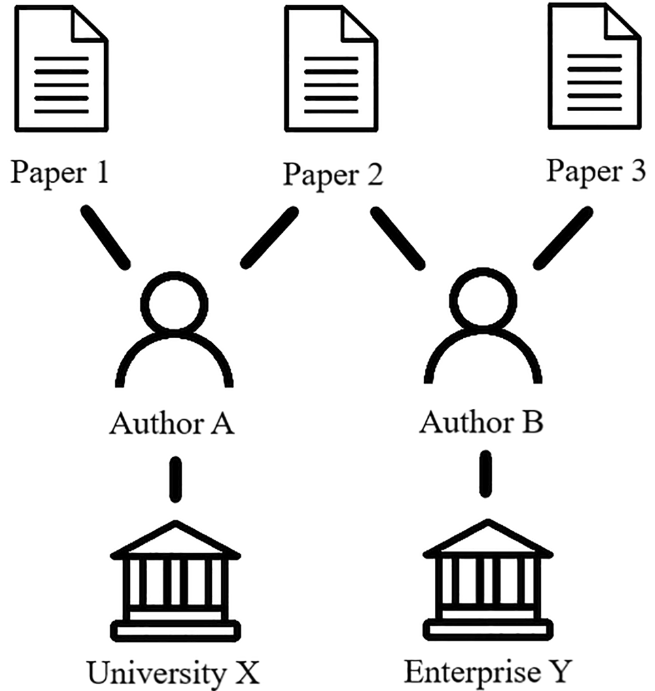
\includegraphics[width=.95\linewidth]{report/images/affiliation-combination.png}
\caption{Exemplary paper-author-\\
affiliation combinations [1]}
\label{fig:affiliation-combination}
\vspace{-50pt}
\end{wrapfigure}
To analyse our research question, we categorize each paper based on the affiliations of its authors, as illustrated in Figure \ref{fig:affiliation-combination}. For each paper, we examine the affiliations of all contributing authors to determine the proportion attributed to corporate entities versus academic institutions.




Methods (spearman correlation, Mann-Whitney U Test)

\clearpage
\section{Results}
To explore the hypothesis—Do papers from corporate-affiliated researchers have more influence at top-tier computer vision conferences?—we begin by examining the trend in the quantity of corporate-affiliated papers over the years. As shown in Figure \ref{fig:corporate_ratio_graph}, the proportion of corporate-affiliated papers has steadily increased across major computer vision conferences. CVPR, ICCV, WACV, and the combined dataset all exhibit a consistent upward trend, with corporate involvement reaching its highest levels in recent years. However, despite this increase, academia continues to dominate these conferences, as the highest ratio of corporate-affiliated papers remains at 0.47. Additionally, while ICCV and CVPR show relatively higher levels of corporate affiliation, WACV consistently lags behind them in this regard. The Spearman rank correlation results in Table \ref{tab:spearman_results} further support the observation in consistent upward trend in corporate affiliation, with strong positive correlations (coefficients exceeding 0.88) and statistically significant p-values (all below 0.05). These findings illustrate the growing presence of corporate-affiliated research within the academic ecosystem of top-tier computer vision venues.

\begin{figure}[ht]
  \centering
  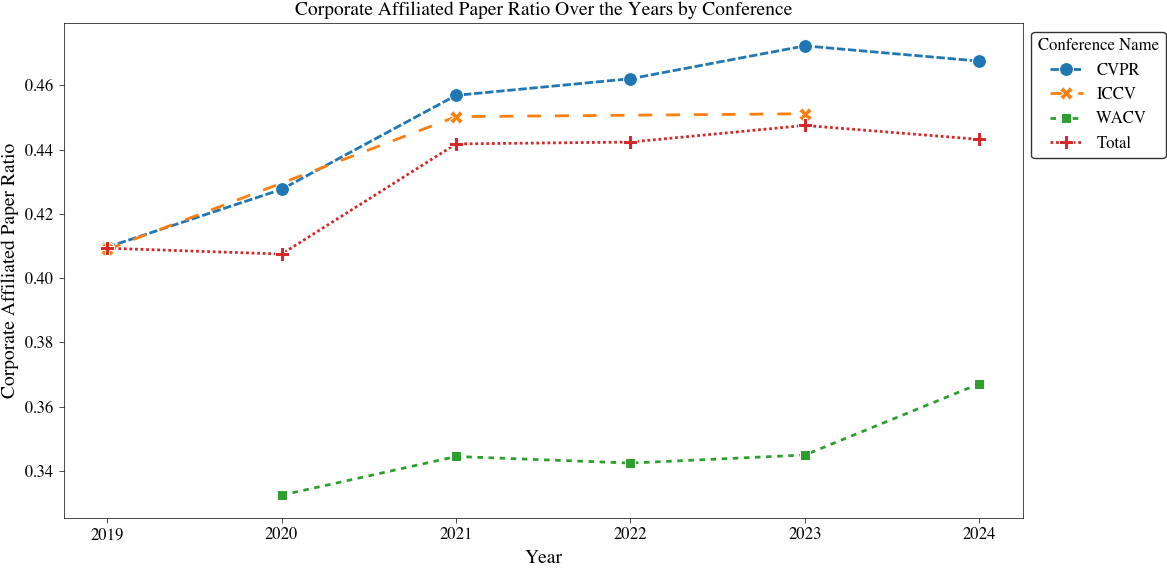
\includegraphics[width=\textwidth]{report/images/corporate_ratio_graph_final.png}  
  \caption{Corporate affiliated paper ratio over the years for each conference and total dataset.}
  \label{fig:corporate_ratio_graph}
\end{figure}

\begin{table}[ht]
\centering
\begin{tabular}{|l|c|c|c|}
\hline
\textbf{Conference} & \textbf{Spearman Correlation} & \textbf{P-value} & \textbf{Significant Relationship?} \\ \hline
CVPR & 0.9429 & 0.0048 & Yes \\ \hline
ICCV & 1.0000 & 0.0000 & Yes \\ \hline
WACV & 0.9000 & 0.0374 & Yes \\ \hline
Total & 0.8857 & 0.0188 & Yes \\ \hline
\end{tabular}
\caption{Spearman rank correlation results for each conference and total dataset.}
\label{tab:spearman_results}
\end{table}

Building on the observed upward trend in the number of corporate-affiliated papers, we now turn our attention to their impact. A critical metric for evaluating research influence is citation count, which reflects the reach and recognition of a paper within the scientific community. To assess this, we compare the citation performance of corporate-affiliated papers to those from academia across top-tier computer vision conferences. Specifically, we examine whether corporate-affiliated papers, despite their lower overall proportion, exhibit higher citation counts, thereby offering insight into their relative impact as hypothesized. We first analyze the distributions of corporate and academia affiliated paper citations. As illustrated in Figure \ref{fig:ieee_citations}, both the number of academia papers and corporate co-authored papers in general have lower citation counts; however, co-authored corporate papers seem to be more prevalent for higher citation counts. The highest citation count (13127) belongs to "Swin Transformer: Hierarchical Vision Transformer using Shifted Windows" authored by Microsoft which makes it an exceptional outlier. To test if corporate affiliated papers have a higher mean citation count ($\mu_2$) than the mean citation of academic papers ($\mu_1$), we perform Mann–Whitney U test. We set $\alpha$ to be 0.05. The null $(H_0)$ and alternative hypothesis $H_\alpha$ are stated below as follows,
\[
H_0 = \mu_2 \leq \mu_1 (\mathrm{Corporate \ papers\ have \ a \ smaller \ or \ equal \ mean \ than \ academia \ ones})
\]
\[
H_\alpha = \mu_2 > \mu_1 (\mathrm{Corporate \ papers\ have \ a \ larger \ mean\ than \ academia \ ones)}
\]
The test results in a p-value of $1.26 \times 10^{-8}$. Thus, we can reject $H_0$, and say that there is a statistically significant difference to indicate that the corporate co-authored papers have a higher IEEE citation mean than academia affiliated papers.   

\begin{figure}
    \centering
    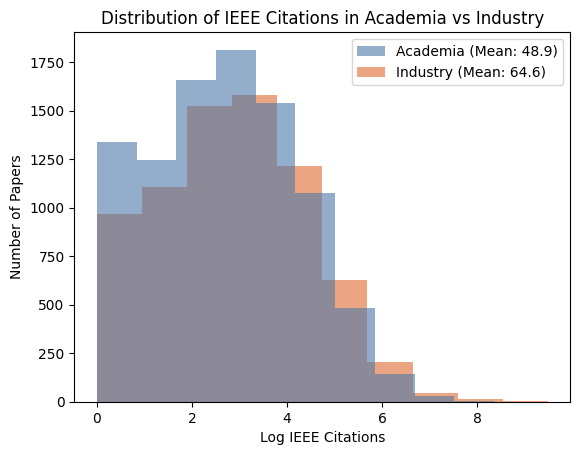
\includegraphics[width=0.6\linewidth]{images/histogram_ieee_citations.png}
    \caption{Distribution of IEEE Citations for Academia and Industry Papers}
    \label{fig:ieee_citations}
\end{figure}

After observing the upward trend in the number of corporate-affiliated papers and their higher IEEE citation counts, it becomes essential to further explore which types of corporations are driving this influence in top-tier computer vision conferences. The dominance of large corporations is particularly striking as shown in Figure \ref{fig:corporate_size_graph}. Big companies contribute over 60\% of corporate representation and nearly 80\% of affiliated papers, solidifying their central role in shaping the research landscape. This is not surprising given that computer vision research often requires immense computational resources, including high-performance hardware, access to large-scale datasets, and advanced machine learning infrastructure—factors that demand significant financial investment. Such resources are more readily available to large corporations, enabling them to produce impactful research and maintain a strong presence in these conferences. The list of the top 10 companies with the highest number of papers—Google, Facebook, Microsoft, Huawei, Adobe, Tencent, Alibaba, Amazon, Nvidia, and Apple—further supports this trend, as all are classified as big companies. 

Notably, these corporations are predominantly based in the USA and China, as reflected in the geographical distribution shown in Figure \ref{fig:corporate_countries}. In contrast, the academic-affiliation choropleth in Figure \ref{fig:academia_countries} reveals a broader, more diverse geographical representation of institutions contributing to computer vision research. Academic institutions from regions worldwide participate in shaping the field, yet there remains significant variability in their research output and influence. This geographical disparity underscores the broader imbalance in resources available to academic institutions compared to corporations.

Smaller organizations, such as scaleups and startups, face additional challenges stemming from this imbalance. Often more geographically dispersed and resource-constrained, these organizations struggle to compete with the financial and computational power of large corporations. This concentration of research output raises critical questions about the extent to which corporate priorities influence the direction of computer vision research. To better understand these dynamics, we analyzed the key research areas explored by corporate and academic-affiliated papers at these top-tier conferences. 


\begin{figure}[ht]
  \centering
  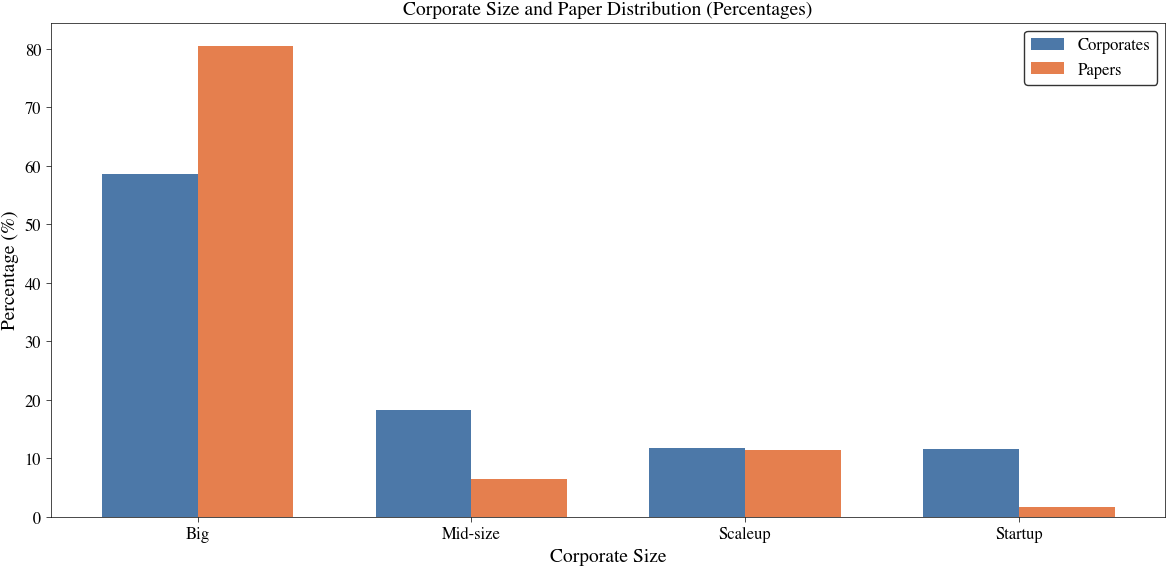
\includegraphics[width=\textwidth]{report/images/corporate_paper_distribution.png}  
  \caption{Corporate size and paper distribution in percentages.}
  \label{fig:corporate_size_graph}
\end{figure}

As illustrated in Figure \ref{fig:research_focus_radar}, Core Vision Algorithms emerge as the dominant research area for both corporate and academic papers, with academia exhibiting a stronger presence, reflecting its emphasis on foundational advancements. Data Collection and Management, the second most prevalent category, receives slightly greater attention from corporate-affiliated research, which aligns with the resource-intensive nature of large-scale data collection—an endeavor where corporations often have a distinct advantage due to their financial and infrastructural capacity. Notably, Mathematical Foundations also rank among the top focus areas, with academia contributing more significantly, yet corporate involvement remains substantial, underscoring the necessity of theoretical advancements even in industry-driven research.

Beyond these core categories, corporate research demonstrates a clear preference for application-oriented fields that align with commercial and industrial interests. Specifically, corporate-affiliated papers exhibit greater attention to Autonomous Vehicles and Robotics, Augmented Reality (AR) and Virtual Reality (VR), Video Analysis and Action Recognition, Generative Models and Creativity, and Natural Language Processing (NLP), all of which represent rapidly growing domains with direct technological applications. Similarly, corporate papers place more emphasis on Datasets and Benchmarks, Industrial and Manufacturing Applications, Human-Centric Vision, and Scene Understanding and Reconstruction, further reflecting corporate interests in scalable, real-world applications of computer vision technologies.

In contrast, academia demonstrates stronger contributions in areas such as Tools and Frameworks and Signal and Statistical Processing—domains that are crucial for developing open-source methodologies, advancing algorithmic efficiency, and refining statistical models for improved interpretability. These findings highlight a distinct contrast between corporate and academic research priorities: while academia continues to drive fundamental innovation, corporate contributions are increasingly shaping the field through resource-intensive, application-driven advancements. This divergence raises important questions about the evolving balance between theoretical exploration and commercially motivated research in computer vision.



\begin{figure}[ht]
  \centering
  \includegraphics[width=\textwidth]{}  
  \caption{Corporate and academia affiliated papers given in categories.}
  \label{fig:research_focus_radar}
\end{figure}

\section{Discussion and Conclusion}
Our study highlights the increasing presence of corporate-affiliated research in top-tier computer vision conferences, with a steady upward trend in corporate contributions. Despite this growth, academia remains dominant, as corporate-affiliated papers have yet to surpass 50\% of total publications. Spearman correlation results confirm this sustained increase, indicating corporate research is becoming a more integral part of the field.

In terms of influence, corporate-affiliated papers exhibit significantly higher citation counts than their academic counterparts, as confirmed by the Mann–Whitney U test. This suggests that industry-backed research has substantial influence, likely due to access to vast computational resources, proprietary datasets, and commercial applications. The dominance of large corporations—such as Google, Facebook, and Microsoft—further underscores this trend, with the majority of corporate-affiliated papers originating from a small set of tech giants. Geographically, corporate research is heavily concentrated in the USA and China, whereas academic contributions exhibit a more globally distributed pattern. This highlights disparities in resources, as smaller organizations, including startups and scaleups, struggle to compete in an increasingly resource-intensive research landscape.

The analysis of research focus areas reveals distinct priorities between academia and corporate. Both emphasize Core Vision Algorithms, but academia places greater focus on Mathematical Foundations and Tools and Frameworks, aligning with fundamental research. In contrast, corporations prioritize applied domains such as Autonomous Vehicles, AR/VR, Video Analysis, and Natural Language Processing, reflecting commercial objectives. Corporates also dedicates more attention to Data Collection and Management, reinforcing its advantage in large-scale datasets.

To ensure a balanced research ecosystem, it is crucial to foster stronger collaborations between academia and industry while preserving the role of fundamental research. Open-access initiatives, shared datasets, and interdisciplinary partnerships could mitigate the risk of research monopolization and maintain a diversity of perspectives in shaping the future of computer vision. Future work should explore the long-term implications of corporate influence on the direction of research, including its impact on funding structures, knowledge dissemination, and ethical considerations surrounding proprietary datasets and closed-source models. Additionally, further investigation into collaboration patterns between academic and corporate researchers may provide insights into how these two sectors can collectively contribute to the advancement of computer vision while maintaining a sustainable and inclusive research environment.
\section{Contributions Statement}
% This is the last section before the references. 

% \emph{Here is an example:}

% XX performed the correlation analysis, organized the data and code for the processing of dataset1 and subdataset2, and created the scatter plot. 
% YY created the random forest regression model, performed the data cleaning for the xyz analysis / xyz database, and created the bar charts to display the regression results. 
% ZZ researched and collected the raw data, restructured the pipeline for the data analysis, and proof-read the draft for the final report. 
% AA performed the data cleaning for dataset1, and performed the Ridge and Lasso regularization. 
% All members of the group contributed to writing the report.

\section*{References}

[1] M. Färber and L. Tampakis, “Analyzing the Impact of Companies on AI Research Based on Publications,” CoRR, vol. abs/2310.20444, 2023, doi: 10.48550/ARXIV.2310.20444.

[2] D. I. Yue, "Google: Estimating the Impact of Corporate Involvement on AI Research," SSRN, Nov. 25, 2024. [Online]. Available: https://ssrn.com/abstract=5033334. doi: 10.2139/ssrn.5033334.

\end{document}
